\documentclass[conference]{IEEEtran}
\usepackage[T1]{fontenc}
\usepackage[utf8]{inputenc}
\usepackage{helvet}
\usepackage{courier}
\usepackage{amssymb}
\usepackage{xcolor}
\usepackage{array}
\usepackage{booktabs}
\usepackage{tikz}
\usepackage{hyperref}
\hypersetup{colorlinks=true,urlcolor=blue!70!black,linkcolor=black,citecolor=black}
\newcommand{\repourl}{\href{https://github.com/DevAbhinav-23/CHIA_Hackathon_2k26}{github.com/DevAbhinav-23/CHIA\_Hackathon\_2k26}}
\usetikzlibrary{shapes.geometric,arrows.meta,positioning,fit,backgrounds,calc}
\usepackage{cite}
\usepackage{microtype}
\usepackage{url}
\usepackage[normalem]{ulem}
\newcommand{\subhead}[1]{\textbf{\uline{#1}:}}
\usepackage{enumitem}
\setlength{\textfloatsep}{6pt plus 2pt minus 2pt}
\setlength{\dbltextfloatsep}{6pt plus 2pt minus 2pt}
\setlength{\floatsep}{7pt plus 2pt minus 2pt}

% ==== figure palette: three hues plus greys, separated by value in greyscale
\definecolor{agF}{HTML}{F6F2FC}\definecolor{agB}{HTML}{6B4FA0} % agent, violet
\definecolor{rbF}{HTML}{A9C4DC}\definecolor{rbB}{HTML}{2F6FAF} % apparatus, blue
\definecolor{dsF}{HTML}{DCDCE0}\definecolor{dsB}{HTML}{9A9AA0} % discarded, grey
\definecolor{hgB}{HTML}{3E6B52}                                % human, green
\definecolor{dgrey}{HTML}{555555}\definecolor{fgrey}{HTML}{7A7A7A}

\begin{document}

\title{From Mined Fixes to Gated Repair:\\Closed-Loop Defect Synthesis for CIRCT}

\author{
  Abhinav Venkata Kota, Adithya Jillellamudi, Priyesh Shukla \\
  International Institute of Information Technology, Hyderabad \\
  \{abhinav.kota, adithya.jillellamudi\}@students.iiit.ac.in, priyesh.shukla@iiit.ac.in
}

\maketitle

\begin{abstract}
A bug in a hardware compiler such as CIRCT can put a silent defect into a chip.
Repair agents fix the bugs people report, but people report few. We built a
closed loop on the CHIA agent framework that supplies its own bugs: a model
reads each of 187 past CIRCT fixes, % 187 fix-shaped commits over 24 months: analysis/pin-window-analysis.md
states the mistake behind it, and writes inputs that probe for the same mistake
elsewhere. Deterministic tools build, judge, reduce and deduplicate every input,
CHIA's repair chain drafts the patch, and a named person approves every filing.
We also restored the assertions CHIA's published image had compiled out, in
536 of its 555 objects. % 606/606 compile commands -DNDEBUG in the published image (frd-followups A-10); 536 of 555 objects reference the assertion handler: 2026-09-14-image-build.md 4
In two campaigns the loop found fifteen new bugs, each reproduced, minimised,
validated and unmatched against 2,652 issues, % 3 + 12 candidates new -> report: runs f1e4fef5, f0b2ef10, db45ab7b; 2,652-issue mirror: docs/HANDOFF.md 2026-09-15 entries
while a mutation baseline over 2,308 inputs found none. % runs 460b7b48 and 91e58983: 1,154 mutants each, 0 firings
Both campaigns read 205 million tokens, 62\% from cache, and wrote 3.7
million.\par % 204.7 M in, 126.3 M cached (61.7 %), 3.72 M out: ledger_entry tokens_in/tokens_out/cached_tokens, runs f1e4fef5, 73effefc, f0b2ef10, db45ab7b
{\raggedright Code and data: \repourl\par}
\end{abstract}

\begin{IEEEkeywords}
Hardware compilers, Program repair, Test generation, Compiler fuzzing, CIRCT.
\end{IEEEkeywords}

% \begin{IEEEkeywords}
% Hardware compilers, Program repair, Test generation, Compiler fuzzing, CIRCT
% \begin{IEEEkeywords}

% =====================================================================
\section{Introduction}
CIRCT is an open-source compiler for hardware, built on MLIR \cite{mlir}. A
designer describes a circuit in FIRRTL or SystemVerilog, CIRCT lowers it to
Verilog, and synthesis tools turn the Verilog into a chip. A crash is visible;
wrong Verilog passes every tool below the compiler and can reach fabrication.
CIRCT's regression tests run under LLVM's \texttt{lit}.

CHIA \cite{chia} is the agent framework this hackathon builds on. Its CIRCT
issue solver takes a GitHub issue through six phases: assess, reproduce, fix,
run the test suite, repair regressions, and write the pull request. On 16 CIRCT
issues it fixed five, and maintainers merged three. Its bottleneck is supply.
Over the past year CIRCT received 82 bug-labelled issues and closed 65; 101
stay open, at a median age of 911 days (Fig.~\ref{fig:motiv}a). % 82 bug-labelled issues, 65 closed, 101 open, median age 911 d: analysis/measurements/2026-09-13-frd-followups.md M1
A fix that corrects one wrong assumption inside a pass usually leaves the same
assumption at other sites. CIRCT ships no fuzzer to find them, and a naive loop
would miss most of them (Fig.~\ref{fig:motiv}b).

\begin{figure}[!t]
\centering
% fig-motivation.tex -- GENERATED by gen_figs.py; edit the generator.
% (a) 82 opened / 65 closed in 12 months; 101 open, median age 911 d
%     analysis/measurements/2026-09-13-frd-followups.md M1
% (b) about 127 of 187 seeds unreachable from FIRRTL; 171 of 187 exact SDK;
%     published image compiled -DNDEBUG (no handler); ours 536 of 555 objects
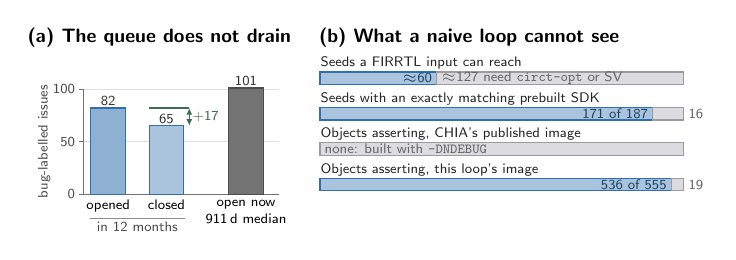
\begin{tikzpicture}[x=1cm,y=1cm]
\node[anchor=south west, inner sep=0pt, font=\sffamily\bfseries\fontsize{6.6}{7.6}\selectfont] at (0.000,1.860) {(a) The queue does not drain};
\draw[line width=0.3pt, draw=black!12] (0.720,0.000) -- (3.200,0.000);
\draw[line width=0.4pt, draw=black!55] (0.660,0.000) -- (0.720,0.000);
\node[anchor=east, inner sep=1pt, font=\sffamily\fontsize{5.5}{6.3}\selectfont, color=black!70] at (0.650,0.000) {0};
\draw[line width=0.3pt, draw=black!12] (0.720,0.667) -- (3.200,0.667);
\draw[line width=0.4pt, draw=black!55] (0.660,0.667) -- (0.720,0.667);
\node[anchor=east, inner sep=1pt, font=\sffamily\fontsize{5.5}{6.3}\selectfont, color=black!70] at (0.650,0.667) {50};
\draw[line width=0.3pt, draw=black!12] (0.720,1.333) -- (3.200,1.333);
\draw[line width=0.4pt, draw=black!55] (0.660,1.333) -- (0.720,1.333);
\node[anchor=east, inner sep=1pt, font=\sffamily\fontsize{5.5}{6.3}\selectfont, color=black!70] at (0.650,1.333) {100};
\draw[line width=0.4pt, draw=black!55] (0.720,0) -- (0.720,1.333);
\draw[line width=0.4pt, draw=black!55] (0.720,0) -- (3.200,0);
\node[rotate=90, anchor=south, inner sep=0pt, font=\sffamily\fontsize{5.5}{6.3}\selectfont, color=black!70] at (0.300,0.667) {bug-labelled issues};
\fill[fill=rbB!55, draw=rbB, line width=0.4pt] (0.810,0) rectangle (1.250,1.093);
\node[anchor=south, inner sep=0.8pt, font=\sffamily\fontsize{5.5}{6.3}\selectfont, color=black!80] at (1.030,1.093) {82};
\fill[fill=rbF, draw=rbB, line width=0.4pt] (1.550,0) rectangle (1.990,0.867);
\node[anchor=south, inner sep=0.8pt, font=\sffamily\fontsize{5.5}{6.3}\selectfont, color=black!80] at (1.770,0.867) {65};
\fill[fill=black!55, draw=black!70, line width=0.4pt] (2.560,0) rectangle (3.000,1.347);
\node[anchor=south, inner sep=0.8pt, font=\sffamily\fontsize{5.5}{6.3}\selectfont, color=black!80] at (2.780,1.347) {101};
\draw[line width=0.4pt, draw=hgB] (1.550,1.093) -- (2.060,1.093);
\draw[line width=0.5pt, draw=hgB, {Latex[length=2.4pt,width=2.2pt]}-{Latex[length=2.4pt,width=2.2pt]}] (2.060,0.867) -- (2.060,1.093);
\node[anchor=west, inner sep=1pt, font=\sffamily\fontsize{5.5}{6.3}\selectfont, color=hgB] at (2.060,0.980) {+17};
\node[anchor=north, align=center, inner sep=0pt, font=\sffamily\fontsize{5.5}{6.3}\selectfont] at (1.030,-0.070) {opened};
\node[anchor=north, align=center, inner sep=0pt, font=\sffamily\fontsize{5.5}{6.3}\selectfont] at (1.770,-0.070) {closed};
\draw[line width=0.3pt, draw=black!45] (0.80,-0.31) -- (2.00,-0.31);
\node[anchor=north, inner sep=0pt, font=\sffamily\fontsize{5.5}{6.3}\selectfont, color=black!70] at (1.40,-0.35) {in 12 months};
\node[anchor=north, align=center, inner sep=0pt, font=\sffamily\fontsize{5.5}{6.3}\selectfont] at (2.780,-0.070) {open now\\911\,d median};
\node[anchor=south west, inner sep=0pt, font=\sffamily\bfseries\fontsize{6.6}{7.6}\selectfont] at (3.700,1.860) {(b) What a naive loop cannot see};
\node[anchor=south west, inner sep=0pt, font=\sffamily\fontsize{5.5}{6.3}\selectfont, color=black!85] at (3.720,1.575) {Seeds a FIRRTL input can reach};
\fill[fill=rbF, draw=rbB, line width=0.4pt] (3.720,1.390) rectangle (5.202,1.550);
\fill[fill=dsF, draw=dsB, line width=0.4pt] (5.202,1.390) rectangle (8.340,1.550);
\node[anchor=east, inner sep=1.5pt, font=\sffamily\fontsize{5.5}{6.3}\selectfont, color=rbB!60!black] at (5.202,1.470) {$\approx$60};
\node[anchor=west, inner sep=1.5pt, font=\sffamily\fontsize{5.5}{6.3}\selectfont, color=black!60] at (5.202,1.470) {$\approx$127 need \texttt{circt-opt} or SV};
\node[anchor=south west, inner sep=0pt, font=\sffamily\fontsize{5.5}{6.3}\selectfont, color=black!85] at (3.720,1.125) {Seeds with an exactly matching prebuilt SDK};
\fill[fill=rbF, draw=rbB, line width=0.4pt] (3.720,0.940) rectangle (7.945,1.100);
\fill[fill=dsF, draw=dsB, line width=0.4pt] (7.945,0.940) rectangle (8.340,1.100);
\node[anchor=east, inner sep=1.5pt, font=\sffamily\fontsize{5.5}{6.3}\selectfont, color=rbB!60!black] at (7.945,1.020) {171 of 187};
\node[anchor=west, inner sep=1.5pt, font=\sffamily\fontsize{5.5}{6.3}\selectfont, color=black!60] at (8.340,1.020) {16};
\node[anchor=south west, inner sep=0pt, font=\sffamily\fontsize{5.5}{6.3}\selectfont, color=black!85] at (3.720,0.675) {Objects asserting, CHIA's published image};
\fill[fill=dsF, draw=dsB, line width=0.4pt] (3.720,0.490) rectangle (8.340,0.650);
\node[anchor=west, inner sep=1.5pt, font=\sffamily\fontsize{5.5}{6.3}\selectfont, color=black!60] at (3.720,0.570) {none: built with \texttt{-DNDEBUG}};
\node[anchor=south west, inner sep=0pt, font=\sffamily\fontsize{5.5}{6.3}\selectfont, color=black!85] at (3.720,0.225) {Objects asserting, this loop's image};
\fill[fill=rbF, draw=rbB, line width=0.4pt] (3.720,0.040) rectangle (8.182,0.200);
\fill[fill=dsF, draw=dsB, line width=0.4pt] (8.182,0.040) rectangle (8.340,0.200);
\node[anchor=east, inner sep=1.5pt, font=\sffamily\fontsize{5.5}{6.3}\selectfont, color=rbB!60!black] at (8.182,0.120) {536 of 555};
\node[anchor=west, inner sep=1.5pt, font=\sffamily\fontsize{5.5}{6.3}\selectfont, color=black!60] at (8.340,0.120) {19};
\end{tikzpicture}

\vspace{-5pt}
\caption{Motivation. (a) CIRCT closes fewer bug issues than it receives,
and what stays open is old. (b) What a mined-fix loop must overcome.}
\label{fig:motiv}
\end{figure}

An agent reads each past fix and writes inputs aimed at those sibling sites,
and tools discard almost everything it writes. Our contributions:
\begin{itemize}
\item A loop in which the model acts three times, reading a fix, writing
  inputs and writing the report, and a tool answers every gate
  (Section~\ref{sec:loop}, Fig.~\ref{fig:loop}).
\item Rebuilds of 171 of 187 historical CIRCT commits in minutes from prebuilt
  SDKs, and an image with assertions restored that passes the same tests
  (Section~\ref{sec:pre}, Table~\ref{tab:meas}).
\item Thresholds pre-registered by git tag, a mutation baseline on the same
  harness, and a dedup rule measured on 22 labelled pairs
  (Section~\ref{sec:eval}).
\item Fifteen new CIRCT bugs through a four-question gate in two campaigns,
  against none from the baseline, every number read from the loop's database
  (Section~\ref{sec:res}, Table~\ref{tab:res}).
\end{itemize}

\begin{figure*}[!t]
\centering
\scalebox{0.78}{% fig-loop.tex -- full-width figure: the attrition ribbon.
% Absolute coordinates in cm. Canvas: x 0.00..18.10, y 1.65..10.70.
% The ribbon's top edge is constant at y=5.50. Its thickness drops at each gate
% and the lost slice peels away downward onto the floor at y=2.50.
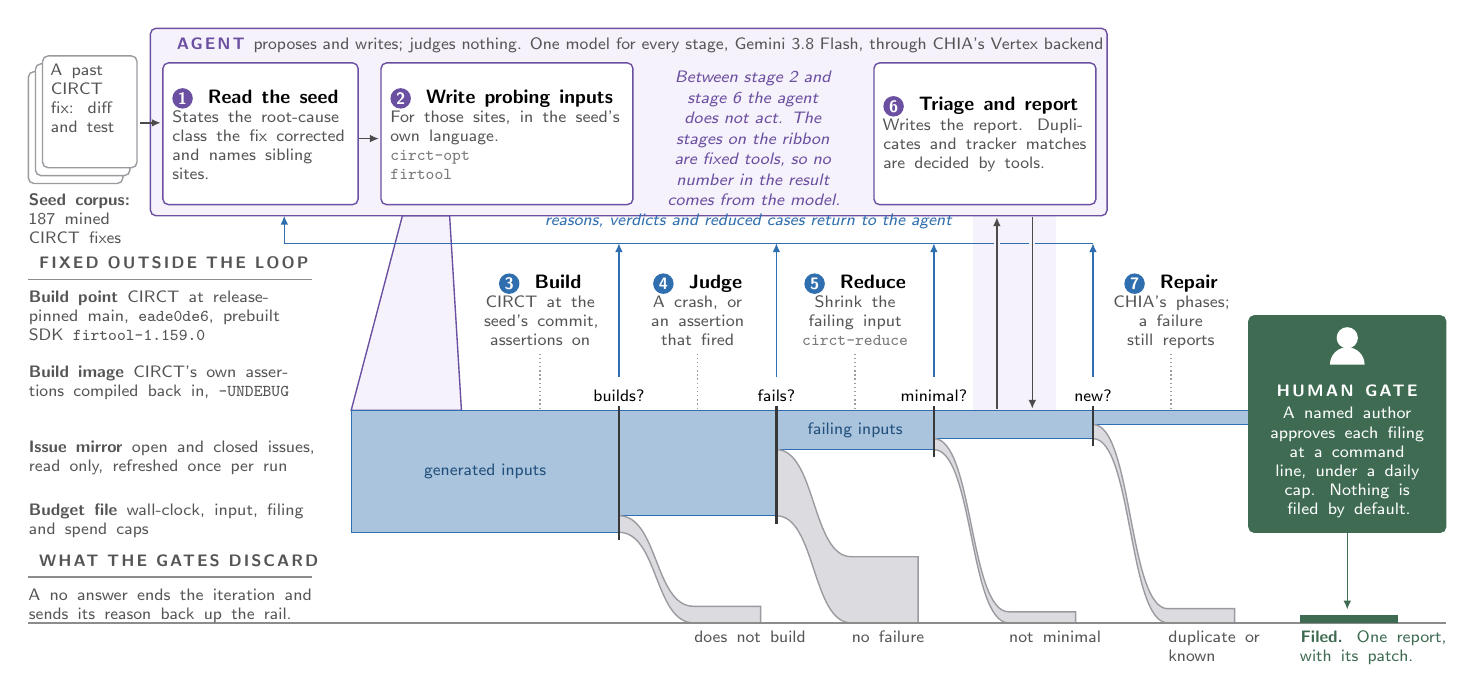
\begin{tikzpicture}[x=1cm,y=1cm,
  font=\sffamily,
  card/.style={draw=agB, fill=white, line width=0.5pt, rounded corners=2pt,
               anchor=north west, align=left, inner xsep=3.4pt, inner ysep=3.4pt},
  blk/.style={anchor=north, align=center, inner sep=1pt},
  txt/.style={anchor=north west, align=left, inner sep=0pt},
  hair/.style={line width=0.5pt, draw=black!45},
  rail/.style={line width=0.5pt, draw=rbB},
  arr/.style={-{Latex[length=3.2pt,width=2.8pt]}, line width=0.5pt, draw=black!70},
  rarr/.style={-{Latex[length=3.2pt,width=2.8pt]}, line width=0.5pt, draw=rbB},
  gatemark/.style={line width=1.0pt, draw=black!78},
  ]

% === type helpers
\newcommand{\ct}[1]{{\sffamily\bfseries\fontsize{7}{7.9}\selectfont #1\par}}
\newcommand{\cd}[1]{{\sffamily\fontsize{6}{6.9}\selectfont\color{dgrey}#1\par}}
\newcommand{\cm}[1]{{\ttfamily\fontsize{6}{6.9}\selectfont\color{fgrey}#1\par}}
\newcommand{\hdr}[1]{{\sffamily\bfseries\fontsize{6.2}{7.2}\selectfont\ifdefined\XeTeXrevision #1\else\textls[110]{#1}\fi}}
\newcommand{\lab}[1]{{\sffamily\fontsize{6}{6.9}\selectfont #1}}
\newcommand{\rlab}[1]{{\sffamily\fontsize{6}{6.9}\selectfont\color{rbB!70!black}#1}}
\newcommand{\nm}[2]{\tikz[baseline=(n.base)]{\node[circle,fill=#2,inner sep=0pt,
   minimum size=7.4pt,anchor=base](n){\textcolor{white}{\sffamily\bfseries
   \fontsize{6}{6}\selectfont\raisebox{-0.4pt}{#1}}};}}
\newcommand{\fx}[4]{\node[txt, text width=3.60cm]
  at (#1,#2) {\cd{\textbf{#3}\ #4}};}

% =============================================== where the agent reaches the flow
% funnel: stage 2 pours generated inputs into the ribbon
\fill[agF, draw=agB, line width=0.5pt]
  (4.80,7.97) -- (5.40,7.97) -- (5.55,5.50) -- (4.15,5.50) -- cycle;
% shaft: the flow rises into stage 6 and comes back down
\fill[agF] (12.05,5.50) rectangle (13.10,7.97);

% ================================================================== agent band
\draw[fill=agF, draw=agB, line width=0.5pt, rounded corners=2pt]
  (1.60,7.97) rectangle (13.75,10.35);
\node[anchor=base west] at (1.80,10.08)
  {{\color{agB}\hdr{AGENT}}\;{\sffamily\fontsize{6.2}{7.2}\selectfont
   \color{dgrey}proposes and writes; judges nothing. One model for every stage,
   Gemini 3.8 Flash, through CHIA's Vertex backend}};
% model and backend: design/ADR/ADR-D-03-model-backend.md, superseding decision 2026-09-14

\node[card, text width=2.24cm, minimum height=1.80cm] at (1.75,9.92)
  {\ct{\nm{1}{agB}\; Read the seed}\cd{States the root-cause class the fix
   corrected and names sibling sites.}};
\node[card, text width=2.96cm, minimum height=1.80cm] at (4.52,9.92)
  {\ct{\nm{2}{agB}\; Write probing inputs}\cd{For those sites, in the seed's own language.}\cm{circt-opt}\cm{firtool}};
\node[card, text width=2.58cm, minimum height=1.80cm] at (10.78,9.92)
  {\ct{\nm{6}{agB}\; Triage and report}\cd{Writes the report. Duplicates and
   tracker matches are decided by tools.}};

\draw[arr] (4.25,8.95) -- (4.50,8.95);

\node[anchor=center, text width=2.42cm, align=center, color=agB,
      font=\sffamily\itshape\fontsize{6.2}{7.4}\selectfont] at (9.25,8.95)
  {Between stage 2 and stage 6 the agent does not act. The stages on the ribbon
   are fixed tools, so no number in the result comes from the model.};

% ================================================================= seed corpus
\foreach \i in {0,1,2}
  {\draw[fill=white, draw=dsB, line width=0.5pt, rounded corners=2pt]
     (0.05+0.09*\i,8.38+0.10*\i) rectangle +(1.20,1.42);}
\node[txt, text width=0.98cm] at (0.33,9.91)
  {\cd{A past CIRCT fix: diff and test}};
\node[txt, text width=1.62cm] at (0.05,8.25)
  {\cd{\textbf{Seed corpus:} 187 mined CIRCT fixes}};
\draw[arr] (1.47,9.15) -- (1.73,9.15);

% ================================================================= return rail
\draw[rail] (13.57,7.62) -- (3.30,7.62);
\draw[rarr] (3.30,7.62) -- (3.30,7.97);
\node[anchor=south east, color=rbB,
      font=\sffamily\itshape\fontsize{6}{7}\selectfont] at (11.90,7.68)
  {reasons, verdicts and reduced cases return to the agent};

% ============================================================ apparatus stages
\node[blk, text width=1.58cm] at (6.55,7.28)
  {\ct{\nm{3}{rbB}\; Build}\cd{CIRCT at the seed's commit, assertions on}};
\node[blk, text width=1.58cm] at (8.55,7.28)
  {\ct{\nm{4}{rbB}\; Judge}\cd{A crash, or an assertion that fired}};
\node[blk, text width=1.58cm] at (10.55,7.28)
  {\ct{\nm{5}{rbB}\; Reduce}\cd{Shrink the failing input}\cm{circt-reduce}};
\node[blk, text width=1.58cm] at (14.56,7.28)
  {\ct{\nm{7}{rbB}\; Repair}\cd{CHIA's phases; a failure still reports}};

\foreach \x in {6.55,8.55,10.55,14.56}
  {\draw[line width=0.5pt, draw=black!38, densely dotted] (\x,6.22) -- (\x,5.52);}

% ======================================================================= ribbon
% segment: from, to, thickness below the constant top edge y=5.50
\foreach \a/\b/\h in {4.15/7.55/1.55, 7.55/9.55/1.34, 9.55/11.55/0.50,
                      11.55/13.57/0.36, 13.57/15.55/0.18}
  {\fill[rbF] (\a,5.50) rectangle (\b,5.50-\h);
   \draw[line width=0.5pt, draw=rbB] (\a,5.50) -- (\b,5.50);
   \draw[line width=0.5pt, draw=rbB] (\a,5.50-\h) -- (\b,5.50-\h);}
\draw[line width=0.5pt, draw=rbB] (4.15,5.50) -- (4.15,3.95);

% what is in flight, named where the ribbon is tall enough to hold the words
\node[anchor=center, inner sep=0pt] at (5.85,4.72) {\rlab{generated inputs}};
\node[anchor=center, inner sep=0pt] at (10.55,5.25) {\rlab{failing inputs}};

% stage 6: the flow rises into the agent and comes back
\draw[arr, preaction={draw, line width=2.2pt, agF}] (12.35,5.52) -- (12.35,7.95);
\draw[arr, preaction={draw, line width=2.2pt, agF}] (12.80,7.95) -- (12.80,5.52);

% ======================================================== gates and what they shed
% gate x, ribbon bottom before, ribbon bottom after, the question
\foreach \g/\bo/\bn/\q in {7.55/3.95/4.16/builds?, 9.55/4.16/5.00/fails?,
                           11.55/5.00/5.14/minimal?, 13.57/5.14/5.32/new?}
  {\fill[dsF, draw=dsB, line width=0.5pt]
     (\g,\bn) .. controls (\g+0.50,\bn) and (\g+0.45,2.80+\bn-\bo) ..
     (\g+0.95,2.80+\bn-\bo) -- (\g+1.80,2.80+\bn-\bo) -- (\g+1.80,2.80)
     -- (\g+0.95,2.80) .. controls (\g+0.45,2.80) and (\g+0.50,\bo) ..
     (\g,\bo) -- cycle;
   \draw[gatemark] (\g,\bo-0.10) -- (\g,5.56);
   \node[anchor=south, inner sep=0.7pt, fill=white] at (\g,5.58) {\lab{\q}};
   \draw[rarr] (\g,5.92) -- (\g,7.62);}

\foreach \g/\l in {7.55/does not build, 9.55/no failure,
                   11.55/not minimal, 13.57/duplicate or known}
  {\node[txt, text width=1.50cm] at (\g+0.95,2.70)
     {\cd{\l}};}

% ======================================================== fixed outside the loop
\node[anchor=base west, color=dgrey] at (0.05,7.30) {\hdr{FIXED OUTSIDE THE LOOP}};
\draw[hair] (0.05,7.16) -- (3.65,7.16);
% build point eade0de6 with SDK firtool-1.159.0: analysis/measurements/2026-09-14-image-build.md 1
\fx{0.05}{7.02}{Build point}{CIRCT at release-pinned main, \texttt{eade0de6}, prebuilt SDK \texttt{firtool-1.159.0}}
\fx{0.05}{6.07}{Build image}{CIRCT's own assertions compiled back in, \texttt{-UNDEBUG}}
\fx{0.05}{5.12}{Issue mirror}{open and closed issues, read only, refreshed once per run}
\fx{0.05}{4.32}{Budget file}{wall-clock, input, filing and spend caps}

% ======================================================================== floor
\draw[hair] (0.05,2.80) -- (18.05,2.80);
\node[anchor=base west, color=dgrey] at (0.05,3.52) {\hdr{WHAT THE GATES DISCARD}};
\draw[hair] (0.05,3.38) -- (3.65,3.38);
\node[txt, text width=3.60cm] at (0.05,3.24)
  {\cd{A no answer ends the iteration and sends its reason back up the rail.}};

% =================================================================== human gate
\draw[fill=hgB, draw=hgB, line width=0.5pt, rounded corners=2pt]
  (15.55,3.95) rectangle (18.05,6.70);
\fill[white] (16.80,6.42) circle (0.135);
\fill[white] (16.58,6.08) arc[start angle=180, end angle=0, radius=0.22] -- cycle;
\node[anchor=north, text width=2.22cm, align=center, color=white] at (16.80,5.94)
  {\hdr{HUMAN GATE}};
\node[anchor=north, text width=2.22cm, align=center, color=white] at (16.80,5.66)
  {{\sffamily\fontsize{6}{6.9}\selectfont A named author approves each filing at
   a command line, under a daily cap. Nothing is filed by default.\par}};

\draw[arr, draw=hgB] (16.80,3.95) -- (16.80,2.97);
\fill[hgB] (16.20,2.80) rectangle (17.45,2.90);
\node[txt, text width=1.85cm] at (16.20,2.70)
  {{\sffamily\fontsize{6}{6.9}\selectfont\color{hgB}\textbf{Filed.} One report,
   with its patch.\par}};

\end{tikzpicture}
}
\caption{Seeded CIRCT bug loop. The agent holds the violet band and acts three
times only, at stages 1, 2 and 6. The blue ribbon below it is fixed apparatus,
so no number in the result comes from the model. The ribbon is the candidates in
flight, pinched at each gate by a yes-or-no question, and the share answering no
peels onto the floor. Widths are illustrative.}
\label{fig:loop}
\end{figure*}

% =====================================================================
\section{The Loop}\label{sec:loop}
Fig.~\ref{fig:loop} marks the stages the agent runs; tools decide everything
else. One model serves every agent stage, Gemini 3.8 Flash through CHIA's
Vertex backend, % model and backend, express mode: design/ADR/ADR-D-03-model-backend.md, superseding decision 2026-09-14
and no stage can reach it unless the operator sets one environment variable for
that run, so tests and dry runs never call the model. % live-call interlock BUGLOOP_ALLOW_LIVE_MODEL: ADR-D-03 rule (1); design/03-LLD.md 3.5.1

\begin{enumerate}[leftmargin=*,itemsep=1pt,topsep=2pt]
\item \subhead{Read the seed} A seed is one of 187 CIRCT commits from the last two
years that look like bug fixes, with its diff and the test its author added or
changed. The agent states which root-cause class the fix corrected and names
other sites where the same assumption still stands. % the SeedRecord carries that diff and those tests, so the worker needs no clone: design/00-README.md, seam rule
\item \subhead{Write probing inputs} The seed's test command names the tool
that reached the bug, \texttt{circt-opt}, \texttt{firtool} or the
SystemVerilog front end, and so decides the language. About 127 of the 187
seeds sit in code no FIRRTL input can reach. The agent reads the compiler's
source through its own tools and runs no command.
\item \subhead{Build} CIRCT compiles against one pinned LLVM and MLIR commit
(Section~\ref{sec:pre}), with CIRCT's assertions compiled in.
\item \subhead{Judge} The primary oracle is unambiguous: the compiler crashed,
or an assertion fired. A second oracle compares CIRCT's simulator with
Verilator and only reports, because the two routinely disagree over
uninitialised and reset signals.
\item \subhead{Reduce} \texttt{circt-reduce}, which CIRCT ships, deletes parts
of a failing input while the failure survives; a textual reducer takes over
where that tool dies.
\item \subhead{Triage and report} A fingerprint is the assertion text with its
source location or, for a crash, the symbolised frames below the crash
handler. It matches survivors against a mirror of CIRCT's issues and against
commits since the build point. The agent writes the report, and no gate reads
what it concluded. % gate reads no triage classification: design/03-LLD.md 3.9 (FR-13.4)
\item \subhead{Repair} CHIA's phase chain runs unaltered except for one branch
that selects our backend and an entry point that takes a local report in place
of a GitHub issue. Repair is restricted to crashes and assertion failures.
\end{enumerate}

\subhead{The gates} Each gate is a yes-or-no question, a bar pinching the
ribbon in Fig.~\ref{fig:loop}; a no returns its reason to the agent with the
verdicts and reduced cases. The last gate asks four questions, each answered by
a tool: does the failure reproduce in a fresh process on another worker, is the
case minimal, is the input valid, and is it new. % four mechanical gate questions: design/03-LLD.md 3.9 (FR-13.1)
Validity is three parse-and-verify commands; a clean rejection makes the input
the loop's fault, not the compiler's. % gate question 3, the three commands: design/03-LLD.md 4.8 (FR-13.15)
Then a named author approves every filing at a command line; by default the
loop files nothing. % approval CLI, python -m circt_bug_loop.approve: design/03-LLD.md 16.2, 13.2 errata

\begin{table}[!t]
\caption{What we measured on the image the loop runs}
\label{tab:meas}
\centering
\scriptsize
\renewcommand{\arraystretch}{0.90}
\begin{tabular}{@{}>{\raggedright\arraybackslash}p{5.55cm}@{\hspace{5pt}}>{\raggedright\arraybackslash}p{2.04cm}@{}}
\toprule
Measurement & Result \\
\midrule
\multicolumn{2}{@{}l}{\textit{Building the past cheaply}}\\
% 187 and 171: analysis/pin-window-analysis.md
Fix-shaped commits mined from 24 months & 187 \\
Of those, seeds with an exactly matching prebuilt SDK & 171 \\
% 16 of 63, worst run 100 commits / 16.1 d: design/ADR/ADR-D-10-lag-window-policy.md, Context
Pin windows with no matching release, worst 16 days & 16 of 63 \\
\addlinespace[2pt]
\multicolumn{2}{@{}l}{\textit{Letting the compiler complain}}\\
% 778 of 778 carry -UNDEBUG, 0 carry -DNDEBUG: analysis/measurements/2026-09-14-image-build.md 4, FR-03.4
Compile commands carrying \texttt{-UNDEBUG} & 778 of 778 \\
% 536 of 555 objects (96.58%): analysis/measurements/2026-09-14-image-build.md 4, FR-03.5
Object files carrying the assertion handler again & 536 of 555 \\
% 1119 passed, 0 failed of 1127 considered, identical in both images: 2026-09-14-image-build.md 5 run 2, and W-04b 3
CHIA's whole test gate, assertions on and then off & 1{,}119 pass, 0 fail, identical \\
% +179 s = 18.4% of wall; +24.48% over six targets; median +4.84% per probe: W-04b 1, 2, 4
What the assertions cost: wall clock, bytes, per probe & 18\%, 25\%, 4\% \\
% lit discovers 1,390 tests with 0 parse errors once MLIR_SOURCE_DIR is the SDK: 2026-09-14-image-build.md 4 (FR-03.17)
Tests \texttt{lit} discovers, once its source root is the SDK & 1{,}390, 0 errors \\
\bottomrule
\end{tabular}
\end{table}

% =====================================================================
\section{Measured Preconditions}\label{sec:pre}
The loop must build CIRCT at arbitrary points of its history, with assertions
on. Neither held when we started; Table~\ref{tab:meas} lists what we measured
on the image the loop now runs.

\subhead{Building the past cheaply} CIRCT pins the exact LLVM commit it
expects; a build against any other fails, and compiling that LLVM costs hours
per seed. CIRCT also publishes prebuilt LLVM and MLIR SDKs carrying their own
pin, and where the two pins match, CIRCT rebuilds in minutes: 171 of the 187
seeds do. The loop itself runs at release-pinned main, the newest commit whose
pin has a published release, 8 commits and 4.8 days behind head for this
image. % lag measured at eade0de6 with SDK firtool-1.159.0: analysis/measurements/2026-09-14-image-build.md 1; ADR-D-10 first application
A longer lag means more candidates come back already fixed.

\subhead{Letting the compiler complain} CHIA's published CIRCT image defines
\texttt{NDEBUG}, which deletes assertions, so an assertion oracle would find
nothing under it. The flag \texttt{-UNDEBUG} puts them back; the 19 objects
without the handler assert nothing. % 536 of 555 objects reference the handler: analysis/measurements/2026-09-14-image-build.md 4, FR-03.5
We built the image twice, differing in that flag alone, and ran CHIA's whole
test gate in both: the same 1,119 tests pass and none fail, % 1,119 of 1,127 considered, 0 failed, identical in both images: image-build.md 5 run 2 and W-04b 3
so a probe that trips an assertion trips it because of the probe. One defect
needed repair first: at CIRCT commits after mid-2026 a test directory's
configuration raises during \texttt{lit} discovery, CHIA's exclusion of that
directory hid the error, and the gate discovered nothing. Using the SDK as the
MLIR source root restores discovery. % MLIR_SOURCE_DIR fix, 1,390 tests discovered: 2026-09-14-image-build.md 4

\subhead{Tested on real failures} We calibrated the oracle and fingerprints on
six past CIRCT bugs, rebuilt at the commit before their fix. % six fixtures, three classes, two SDK tags, build costs 14 s to 601 s: analysis/measurements/2026-09-14-crash-fixtures.md 1 and 2
This exposed two fingerprinting defects: the name normaliser erased every frame
in an anonymous namespace, where CIRCT's passes live, and the scope test read
an inlined frame instead of the physical one. Together they put three of the
four real bugs outside the repair stage's reach; we fixed both. % the two frame defects: 2026-09-14-crash-fixtures.md 3.2 and 3.4; design/reviews/implementation-errata-log.md W-08 rows 1 and 2

% =====================================================================
\section{Controls}\label{sec:eval}
The question is whether reading a past fix finds more new bugs than mutating
the same tests. Two arms share the harness, oracles, reducer and gate; only the
generator and its information differ. The mutation arm rewrites seed tests
syntactically, on 96 of the 184 eligible seeds, without the diff or the
root-cause class, after Mut4All's model-synthesised mutators \cite{mut4all}.
Both arms get the same wall-clock window, but the mutation arm exhausts its
mutants after 775 and 266 seconds; a post-review run that used the whole window
gated 2 bugs from 115,869 inputs. The registered headline is distinct bugs a
CIRCT maintainer confirms by labelling, commenting on or fixing them; until
filing, we report bugs through the gate.

\subhead{Pre-registration} Every threshold lives in one budget file, registered
by an annotated git tag on the commit that lands it. The loop refuses an
untagged file and a mutator set committed after the tag. % registration/<run> tag, load_budget checks, mutator set must be an ancestor: circt_bug_loop/budget.py; docs/HANDOFF.md W-12b
Safety caps bound damage: 2,000 inputs per arm per day, 3 filings per day and
10 per run, 60 seconds and 4\,GiB per probe, and a hard cap on model
spending. % the caps: circt_bug_loop/budget.yaml
Nothing is filed until a human has posted the method to the project's
forum. % FR-20.1 enforced at approval (python -m circt_bug_loop.approve), FR-20.2

\subhead{Deduplication} Two candidates are one bug when their primary
fingerprints are equal. On 22 hand-labelled pairs the rule merges 1 of the 11
distinct pairs and splits 1 of the 11 duplicates. % 22 labelled pairs, collision 1/11, false merge 1/11: design/reviews/implementation-errata-log.md W-10 row 20

\subhead{Known issues} GitHub stops paginating at page 100, so the tracker
mirror walks newest first, then oldest first, and unions the two: 2,652 issues
in 198 requests. % 422 at page 100: implementation-errata-log.md W-14 row 21; live mirror 2,652 issues (1,795 closed / 857 open), 198 pages, 200 s: docs/HANDOFF.md W-17 join

\subhead{Contamination} The model may have memorised later CIRCT fixes. We
screen each candidate against fixes made after its seed, at the level of the
symbols the seed's fix touched; this flags 77\% of the corpus, against 96\% at
file level. % symbol level 77.0%, file level 96.3%: analysis/measurements/2026-09-13-frd-followups.md M4
A flag marks a candidate and does not exclude it.

% =====================================================================
\section{Results}\label{sec:res}
Table~\ref{tab:res} reports two registered campaigns, each running the seeded
arm as two parallel shards. The first gave every arm two hours under a
per-job spending cap; we stopped its first two starts early for defects the
live run exposed. % registration/campaign-2 on cb75a0f; docs/HANDOFF.md 2026-09-15 06:05 and 07:05 entries
The second changed only three registered numbers: the whole corpus, a
41.7-hour window and a higher cap. We stopped it after 11.9 hours. % registration/campaign-3 on a65331b; launched 19:01 UTC, stopped 06:54:56 UTC
Every number comes from the loop's database after re-judging stored probes
under the corrections below, with no model turn re-run. % --reclassify and --rescreen, head-only, no model turn

\begin{table}[!t]
\caption{Both campaigns, from the loop's database. A seeded column is its two
shards together. The mutation column is one run per campaign, and the two runs
agree in every cell}
\label{tab:res}
\centering
\scriptsize
\renewcommand{\arraystretch}{0.90}
\begin{tabular}{@{}>{\raggedright\arraybackslash}p{3.65cm}@{\hspace{4pt}}>{\centering\arraybackslash}p{1.15cm}@{\hspace{4pt}}>{\centering\arraybackslash}p{1.15cm}@{\hspace{4pt}}>{\centering\arraybackslash}p{1.15cm}@{}}
\toprule
Measure & seeded 1 & seeded 2 & mutation \\
\midrule
% campaign_aggregate.py: f1e4fef5+73effefc, f0b2ef10+db45ab7b, 460b7b48 = 91e58983
Seeds probed & 9 & 43 & 96 \\
Probes written & 134 & 624 & 1{,}154 \\
Output rejected by its own verifier & 10 & 7 & 0 \\
Assertion failures & 5 & 54 & 0 \\
Crashes & 0 & 8 & 0 \\
Candidates & 15 & 69 & 0 \\
Distinct new fingerprints & 3 & 14 & 0 \\
Through the gate & 3 & 12 & 0 \\
Filed & 0 & 0 & 0 \\
% 57 and 191 metered turns carrying a call count (the 57 include the three stage-6 report turns of f1e4fef5)
Model turns & 57 & 191 & 0 \\
% tokens_in: 56,034,371 and 148,709,459; tokens_out: 723,615 and 2,995,789; cached 37,901,964 (67.6%) and 88,433,498 (59.5%)
Input tokens, millions (share from cache) & 56.0 (68\%) & 148.7 (59\%) & 0 \\
Output tokens, millions & 0.72 & 3.00 & 0 \\
\bottomrule
\end{tabular}
\end{table}

\begin{figure*}[!t]
\centering
% fig-analysis.tex -- GENERATED by gen_figs.py; edit the generator.
% Values: Table II of main.tex and ratios of its cells; (d) from W-04b 1,2,4.
%  (a) seeded 134+624=758 inputs, 15+69=84 cand., 3+14=17 fp, 3+12=15 gated;
%      mutation 2 x 1,154 = 2,308 inputs and 0 everywhere else
%  (b) 15/134=11.2, 69/624=11.1, 3/134=2.2, 12/624=1.9 per 100 inputs
%  (c) 44.49/9=4.9, 122.77/43=2.9 per seed; 44.49/3=14.8, 122.77/12=10.2 per bug
%  (d) +18.4% wall, +24.5% bytes, +4.8% median per probe
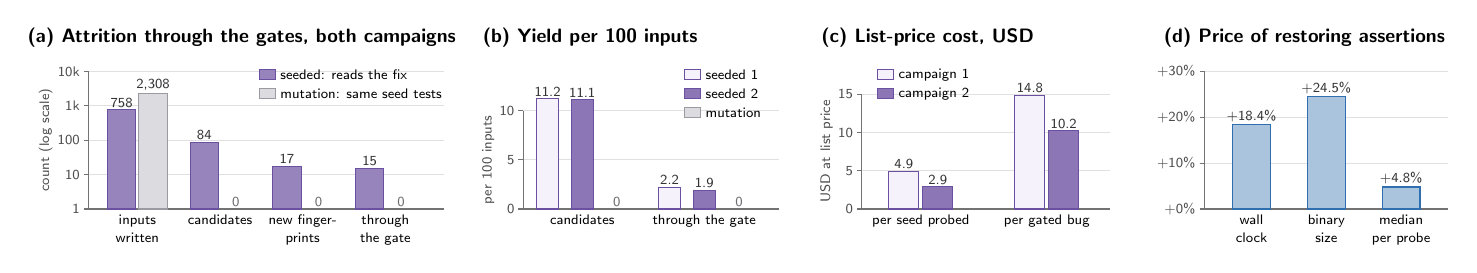
\begin{tikzpicture}[x=1cm,y=1cm]
\node[anchor=south west, inner sep=0pt, font=\sffamily\bfseries\fontsize{6.6}{7.6}\selectfont] at (0.000,2.050) {(a) Attrition through the gates, both campaigns};
\draw[line width=0.3pt, draw=black!12] (0.780,0.000) -- (5.300,0.000);
\draw[line width=0.4pt, draw=black!55] (0.720,0.000) -- (0.780,0.000);
\node[anchor=east, inner sep=1pt, font=\sffamily\fontsize{5.5}{6.3}\selectfont, color=black!70] at (0.710,0.000) {1};
\draw[line width=0.3pt, draw=black!12] (0.780,0.438) -- (5.300,0.438);
\draw[line width=0.4pt, draw=black!55] (0.720,0.438) -- (0.780,0.438);
\node[anchor=east, inner sep=1pt, font=\sffamily\fontsize{5.5}{6.3}\selectfont, color=black!70] at (0.710,0.438) {10};
\draw[line width=0.3pt, draw=black!12] (0.780,0.875) -- (5.300,0.875);
\draw[line width=0.4pt, draw=black!55] (0.720,0.875) -- (0.780,0.875);
\node[anchor=east, inner sep=1pt, font=\sffamily\fontsize{5.5}{6.3}\selectfont, color=black!70] at (0.710,0.875) {100};
\draw[line width=0.3pt, draw=black!12] (0.780,1.312) -- (5.300,1.312);
\draw[line width=0.4pt, draw=black!55] (0.720,1.312) -- (0.780,1.312);
\node[anchor=east, inner sep=1pt, font=\sffamily\fontsize{5.5}{6.3}\selectfont, color=black!70] at (0.710,1.312) {1k};
\draw[line width=0.3pt, draw=black!12] (0.780,1.750) -- (5.300,1.750);
\draw[line width=0.4pt, draw=black!55] (0.720,1.750) -- (0.780,1.750);
\node[anchor=east, inner sep=1pt, font=\sffamily\fontsize{5.5}{6.3}\selectfont, color=black!70] at (0.710,1.750) {10k};
\draw[line width=0.4pt, draw=black!55] (0.780,0) -- (0.780,1.750);
\draw[line width=0.4pt, draw=black!55] (0.780,0) -- (5.300,0);
\node[rotate=90, anchor=south, inner sep=0pt, font=\sffamily\fontsize{5.5}{6.3}\selectfont, color=black!70] at (0.330,0.875) {count (log scale)};
\fill[fill=agB!70, draw=agB, line width=0.4pt] (1.020,0) rectangle (1.380,1.260);
\node[anchor=south, inner sep=0.8pt, font=\sffamily\fontsize{5.5}{6.3}\selectfont, color=black!80] at (1.200,1.260) {758};
\fill[fill=dsF, draw=dsB, line width=0.4pt] (1.420,0) rectangle (1.780,1.471);
\node[anchor=south, inner sep=0.8pt, font=\sffamily\fontsize{5.5}{6.3}\selectfont, color=black!80] at (1.600,1.471) {2{,}308};
\node[anchor=north, align=center, inner sep=0pt, font=\sffamily\fontsize{5.5}{6.3}\selectfont] at (1.400,-0.070) {inputs\\written};
\fill[fill=agB!70, draw=agB, line width=0.4pt] (2.070,0) rectangle (2.430,0.842);
\node[anchor=south, inner sep=0.8pt, font=\sffamily\fontsize{5.5}{6.3}\selectfont, color=black!80] at (2.250,0.842) {84};
\node[anchor=south, inner sep=0.8pt, font=\sffamily\fontsize{5.5}{6.3}\selectfont, color=dsB!70!black] at (2.650,0.000) {0};
\node[anchor=north, align=center, inner sep=0pt, font=\sffamily\fontsize{5.5}{6.3}\selectfont] at (2.450,-0.070) {candidates};
\fill[fill=agB!70, draw=agB, line width=0.4pt] (3.120,0) rectangle (3.480,0.538);
\node[anchor=south, inner sep=0.8pt, font=\sffamily\fontsize{5.5}{6.3}\selectfont, color=black!80] at (3.300,0.538) {17};
\node[anchor=south, inner sep=0.8pt, font=\sffamily\fontsize{5.5}{6.3}\selectfont, color=dsB!70!black] at (3.700,0.000) {0};
\node[anchor=north, align=center, inner sep=0pt, font=\sffamily\fontsize{5.5}{6.3}\selectfont] at (3.500,-0.070) {new finger-\\prints};
\fill[fill=agB!70, draw=agB, line width=0.4pt] (4.170,0) rectangle (4.530,0.515);
\node[anchor=south, inner sep=0.8pt, font=\sffamily\fontsize{5.5}{6.3}\selectfont, color=black!80] at (4.350,0.515) {15};
\node[anchor=south, inner sep=0.8pt, font=\sffamily\fontsize{5.5}{6.3}\selectfont, color=dsB!70!black] at (4.750,0.000) {0};
\node[anchor=north, align=center, inner sep=0pt, font=\sffamily\fontsize{5.5}{6.3}\selectfont] at (4.550,-0.070) {through\\the gate};
\fill[fill=agB!70, draw=agB, line width=0.4pt] (2.950,1.640) rectangle (3.150,1.770);
\node[anchor=west, inner sep=0pt, font=\sffamily\fontsize{5.5}{6.3}\selectfont] at (3.210,1.700) {seeded: reads the fix};
\fill[fill=dsF, draw=dsB, line width=0.4pt] (2.950,1.400) rectangle (3.150,1.530);
\node[anchor=west, inner sep=0pt, font=\sffamily\fontsize{5.5}{6.3}\selectfont] at (3.210,1.460) {mutation: same seed tests};
\node[anchor=south west, inner sep=0pt, font=\sffamily\bfseries\fontsize{6.6}{7.6}\selectfont] at (5.780,2.050) {(b) Yield per 100 inputs};
\draw[line width=0.3pt, draw=black!12] (6.300,0.000) -- (9.550,0.000);
\draw[line width=0.4pt, draw=black!55] (6.240,0.000) -- (6.300,0.000);
\node[anchor=east, inner sep=1pt, font=\sffamily\fontsize{5.5}{6.3}\selectfont, color=black!70] at (6.230,0.000) {0};
\draw[line width=0.3pt, draw=black!12] (6.300,0.625) -- (9.550,0.625);
\draw[line width=0.4pt, draw=black!55] (6.240,0.625) -- (6.300,0.625);
\node[anchor=east, inner sep=1pt, font=\sffamily\fontsize{5.5}{6.3}\selectfont, color=black!70] at (6.230,0.625) {5};
\draw[line width=0.3pt, draw=black!12] (6.300,1.250) -- (9.550,1.250);
\draw[line width=0.4pt, draw=black!55] (6.240,1.250) -- (6.300,1.250);
\node[anchor=east, inner sep=1pt, font=\sffamily\fontsize{5.5}{6.3}\selectfont, color=black!70] at (6.230,1.250) {10};
\draw[line width=0.4pt, draw=black!55] (6.300,0) -- (6.300,1.250);
\draw[line width=0.4pt, draw=black!55] (6.300,0) -- (9.550,0);
\node[rotate=90, anchor=south, inner sep=0pt, font=\sffamily\fontsize{5.5}{6.3}\selectfont, color=black!70] at (5.940,0.625) {per 100 inputs};
\fill[fill=agF, draw=agB, line width=0.4pt] (6.470,0) rectangle (6.750,1.400);
\node[anchor=south, inner sep=0.8pt, font=\sffamily\fontsize{5.5}{6.3}\selectfont, color=black!80] at (6.610,1.400) {11.2};
\fill[fill=agB!78, draw=agB, line width=0.4pt] (6.910,0) rectangle (7.190,1.387);
\node[anchor=south, inner sep=0.8pt, font=\sffamily\fontsize{5.5}{6.3}\selectfont, color=black!80] at (7.050,1.387) {11.1};
\node[anchor=south, inner sep=0.8pt, font=\sffamily\fontsize{5.5}{6.3}\selectfont, color=dsB!70!black] at (7.490,0.000) {0};
\node[anchor=north, align=center, inner sep=0pt, font=\sffamily\fontsize{5.5}{6.3}\selectfont] at (7.050,-0.070) {candidates};
\fill[fill=agF, draw=agB, line width=0.4pt] (8.020,0) rectangle (8.300,0.275);
\node[anchor=south, inner sep=0.8pt, font=\sffamily\fontsize{5.5}{6.3}\selectfont, color=black!80] at (8.160,0.275) {2.2};
\fill[fill=agB!78, draw=agB, line width=0.4pt] (8.460,0) rectangle (8.740,0.237);
\node[anchor=south, inner sep=0.8pt, font=\sffamily\fontsize{5.5}{6.3}\selectfont, color=black!80] at (8.600,0.237) {1.9};
\node[anchor=south, inner sep=0.8pt, font=\sffamily\fontsize{5.5}{6.3}\selectfont, color=dsB!70!black] at (9.040,0.000) {0};
\node[anchor=north, align=center, inner sep=0pt, font=\sffamily\fontsize{5.5}{6.3}\selectfont] at (8.600,-0.070) {through the gate};
\fill[fill=agF, draw=agB, line width=0.4pt] (8.350,1.640) rectangle (8.550,1.770);
\node[anchor=west, inner sep=0pt, font=\sffamily\fontsize{5.5}{6.3}\selectfont] at (8.610,1.700) {seeded 1};
\fill[fill=agB!78, draw=agB, line width=0.4pt] (8.350,1.400) rectangle (8.550,1.530);
\node[anchor=west, inner sep=0pt, font=\sffamily\fontsize{5.5}{6.3}\selectfont] at (8.610,1.460) {seeded 2};
\fill[fill=dsF, draw=dsB, line width=0.4pt] (8.350,1.160) rectangle (8.550,1.290);
\node[anchor=west, inner sep=0pt, font=\sffamily\fontsize{5.5}{6.3}\selectfont] at (8.610,1.220) {mutation};
\node[anchor=south west, inner sep=0pt, font=\sffamily\bfseries\fontsize{6.6}{7.6}\selectfont] at (10.080,2.050) {(c) List-price cost, USD};
\draw[line width=0.3pt, draw=black!12] (10.600,0.000) -- (13.750,0.000);
\draw[line width=0.4pt, draw=black!55] (10.540,0.000) -- (10.600,0.000);
\node[anchor=east, inner sep=1pt, font=\sffamily\fontsize{5.5}{6.3}\selectfont, color=black!70] at (10.530,0.000) {0};
\draw[line width=0.3pt, draw=black!12] (10.600,0.486) -- (13.750,0.486);
\draw[line width=0.4pt, draw=black!55] (10.540,0.486) -- (10.600,0.486);
\node[anchor=east, inner sep=1pt, font=\sffamily\fontsize{5.5}{6.3}\selectfont, color=black!70] at (10.530,0.486) {5};
\draw[line width=0.3pt, draw=black!12] (10.600,0.972) -- (13.750,0.972);
\draw[line width=0.4pt, draw=black!55] (10.540,0.972) -- (10.600,0.972);
\node[anchor=east, inner sep=1pt, font=\sffamily\fontsize{5.5}{6.3}\selectfont, color=black!70] at (10.530,0.972) {10};
\draw[line width=0.3pt, draw=black!12] (10.600,1.458) -- (13.750,1.458);
\draw[line width=0.4pt, draw=black!55] (10.540,1.458) -- (10.600,1.458);
\node[anchor=east, inner sep=1pt, font=\sffamily\fontsize{5.5}{6.3}\selectfont, color=black!70] at (10.530,1.458) {15};
\draw[line width=0.4pt, draw=black!55] (10.600,0) -- (10.600,1.458);
\draw[line width=0.4pt, draw=black!55] (10.600,0) -- (13.750,0);
\node[rotate=90, anchor=south, inner sep=0pt, font=\sffamily\fontsize{5.5}{6.3}\selectfont, color=black!70] at (10.240,0.729) {USD at list price};
\fill[fill=agF, draw=agB, line width=0.4pt] (10.945,0) rectangle (11.325,0.476);
\node[anchor=south, inner sep=0.8pt, font=\sffamily\fontsize{5.5}{6.3}\selectfont, color=black!80] at (11.135,0.476) {4.9};
\fill[fill=agB!78, draw=agB, line width=0.4pt] (11.375,0) rectangle (11.755,0.282);
\node[anchor=south, inner sep=0.8pt, font=\sffamily\fontsize{5.5}{6.3}\selectfont, color=black!80] at (11.565,0.282) {2.9};
\node[anchor=north, align=center, inner sep=0pt, font=\sffamily\fontsize{5.5}{6.3}\selectfont] at (11.350,-0.070) {per seed probed};
\fill[fill=agF, draw=agB, line width=0.4pt] (12.545,0) rectangle (12.925,1.439);
\node[anchor=south, inner sep=0.8pt, font=\sffamily\fontsize{5.5}{6.3}\selectfont, color=black!80] at (12.735,1.439) {14.8};
\fill[fill=agB!78, draw=agB, line width=0.4pt] (12.975,0) rectangle (13.355,0.992);
\node[anchor=south, inner sep=0.8pt, font=\sffamily\fontsize{5.5}{6.3}\selectfont, color=black!80] at (13.165,0.992) {10.2};
\node[anchor=north, align=center, inner sep=0pt, font=\sffamily\fontsize{5.5}{6.3}\selectfont] at (12.950,-0.070) {per gated bug};
\fill[fill=agF, draw=agB, line width=0.4pt] (10.800,1.640) rectangle (11.000,1.770);
\node[anchor=west, inner sep=0pt, font=\sffamily\fontsize{5.5}{6.3}\selectfont] at (11.060,1.700) {campaign 1};
\fill[fill=agB!78, draw=agB, line width=0.4pt] (10.800,1.400) rectangle (11.000,1.530);
\node[anchor=west, inner sep=0pt, font=\sffamily\fontsize{5.5}{6.3}\selectfont] at (11.060,1.460) {campaign 2};
\node[anchor=south west, inner sep=0pt, font=\sffamily\bfseries\fontsize{6.6}{7.6}\selectfont] at (14.430,2.050) {(d) Price of restoring assertions};
\draw[line width=0.3pt, draw=black!12] (14.950,0.000) -- (18.050,0.000);
\draw[line width=0.4pt, draw=black!55] (14.890,0.000) -- (14.950,0.000);
\node[anchor=east, inner sep=1pt, font=\sffamily\fontsize{5.5}{6.3}\selectfont, color=black!70] at (14.880,0.000) {+0\%};
\draw[line width=0.3pt, draw=black!12] (14.950,0.583) -- (18.050,0.583);
\draw[line width=0.4pt, draw=black!55] (14.890,0.583) -- (14.950,0.583);
\node[anchor=east, inner sep=1pt, font=\sffamily\fontsize{5.5}{6.3}\selectfont, color=black!70] at (14.880,0.583) {+10\%};
\draw[line width=0.3pt, draw=black!12] (14.950,1.167) -- (18.050,1.167);
\draw[line width=0.4pt, draw=black!55] (14.890,1.167) -- (14.950,1.167);
\node[anchor=east, inner sep=1pt, font=\sffamily\fontsize{5.5}{6.3}\selectfont, color=black!70] at (14.880,1.167) {+20\%};
\draw[line width=0.3pt, draw=black!12] (14.950,1.750) -- (18.050,1.750);
\draw[line width=0.4pt, draw=black!55] (14.890,1.750) -- (14.950,1.750);
\node[anchor=east, inner sep=1pt, font=\sffamily\fontsize{5.5}{6.3}\selectfont, color=black!70] at (14.880,1.750) {+30\%};
\draw[line width=0.4pt, draw=black!55] (14.950,0) -- (14.950,1.750);
\draw[line width=0.4pt, draw=black!55] (14.950,0) -- (18.050,0);
\fill[fill=rbF, draw=rbB, line width=0.4pt] (15.310,0) rectangle (15.790,1.073);
\node[anchor=south, inner sep=0.8pt, font=\sffamily\fontsize{5.5}{6.3}\selectfont, color=black!80] at (15.550,1.073) {+18.4\%};
\node[anchor=north, align=center, inner sep=0pt, font=\sffamily\fontsize{5.5}{6.3}\selectfont] at (15.550,-0.070) {wall\\clock};
\fill[fill=rbF, draw=rbB, line width=0.4pt] (16.260,0) rectangle (16.740,1.429);
\node[anchor=south, inner sep=0.8pt, font=\sffamily\fontsize{5.5}{6.3}\selectfont, color=black!80] at (16.500,1.429) {+24.5\%};
\node[anchor=north, align=center, inner sep=0pt, font=\sffamily\fontsize{5.5}{6.3}\selectfont] at (16.500,-0.070) {binary\\size};
\fill[fill=rbF, draw=rbB, line width=0.4pt] (17.210,0) rectangle (17.690,0.280);
\node[anchor=south, inner sep=0.8pt, font=\sffamily\fontsize{5.5}{6.3}\selectfont, color=black!80] at (17.450,0.280) {+4.8\%};
\node[anchor=north, align=center, inner sep=0pt, font=\sffamily\fontsize{5.5}{6.3}\selectfont] at (17.450,-0.070) {median\\per probe};
\end{tikzpicture}

\vspace{-5pt}
\caption{Both registered campaigns (Table~\ref{tab:res}). (a)~One harness,
oracle and gate; only the generator and its information differ. Zeros sit at the log axis
floor. (b)~Rates agree though campaign~2 is five times larger. (c)~Model use
per gated bug at list price, USD 0.75 and 3.75 per million input and output
tokens. (d)~Overheads of Table~\ref{tab:meas}.}
\label{fig:analysis}
\end{figure*}

\subhead{Stable yield} Fig.~\ref{fig:analysis} reads Table~\ref{tab:res} as
rates. The seeded campaigns differ fivefold in size, yet yield 11.2 and 11.1
candidates and 2.2 and 1.9 gated bugs per 100 inputs. The mutation arm wrote
three times as many inputs as both seeded campaigns together and none fired
the oracle; only 34\% reached the pass they target. A gated bug cost 18.7
million input tokens in the first campaign and 12.4 million in the
second. % 56.03 M / 3 and 148.71 M / 12
Fifteen bugs establish a consistent rate, not an effect size.

\subhead{Fifteen new bugs} The first campaign's three all come from the August
\texttt{moore.extract} seed: a zero-element array trips the assertion at
\texttt{HWOps.cpp:1995}, and a dynamic extract and an extract of a reference
lower to \texttt{comb.extract} and \texttt{llhd.sig.extract} with aggregate
types. % candidates c-p-a2cb61b8d0aa, c-p-075cf1d70f3a, c-p-356e9e6e061d; seed cc71d34a
The second campaign's twelve spread across the compiler; three are not
assertions: a segmentation fault in \texttt{resolveClassStructBody} in
\texttt{MooreToCore.cpp}, one whose only named frame is \texttt{main} in
\texttt{circt-opt.cpp}, and an abort in
\texttt{ElaboratedObjectOp::}\allowbreak\texttt{verifySymbolUses} in
\texttt{OMOps.cpp}. % candidates c-p-4d7a36e3ce15, c-p-4b9f84841ec3, c-p-a3a1556793d7
All fifteen passed the four gate questions. % gate q1-q4 per candidate: runs f1e4fef5, f0b2ef10, db45ab7b store
They share twelve root causes. Re-run on CIRCT main of 26 October, built the
same way, all fifteen still fail as the same bug, and no issue or commit since
the pin reports or fixes any of them. % main 4738bd26, firtool-1.162.0 SDK, 277 issues/PRs since 2026-09-16 searched: analysis/measurements/2026-10-27-recheck-main.md; root causes: 2026-10-27-repairs.md
Two more new fingerprints failed the gate: one did not reproduce, and the
validity checker rejected the other. % c-p-0eec26191ff2 unreproducible, c-p-bb144e1c880c invalid_input

\subhead{The oracle had to learn a class} Seventeen rejected seeded probes were
the compiler's fault, not the model's: the input alone parses and verifies,
and the diagnostic has the shape of MLIR's generated verifier. We require both,
since a pass may legitimately reject a valid input, such as one with two
top-level modules. % D-13: probe_task._GENERATED_VERIFIER and the parse-and-verify command; docs/HANDOFF.md 07:55 entry
No mutation rejection qualified: a mutated test that fails to parse is broken
syntax. % runs 460b7b48 and 91e58983

\subhead{Four dedup corrections} Each was found on a real candidate. A
post-pin commit counted as a fix if it touched the crash's file, so an LLVM
bump touching 87 files silenced the first find; it now has to touch a frame
symbol. A generic MLIR assertion text matched an open issue, and now also needs
a CIRCT frame token. A verifier failure matched an issue on the op name alone,
and now needs the constraint. Two candidates sharing a fingerprint were each
the other's duplicate, which left thirteen without a representative. % D-11, D-16, D-17, D-18: docs/HANDOFF.md 2026-09-15 entries
Verdicts are recomputed from stored evidence, so a corrected rule re-judges
every candidate without a model turn.

\subhead{Tokens} The campaigns read about 6.2 and 3.5 million input tokens per
seed. % ledger_entry tokens_in/tokens_out per run
Most of that is re-reading: CHIA's backend resends the whole conversation on
every tool call, so a turn with twelve calls reads its context twelve
times. % quadratic resend measured W-18 (budget.yaml, max_tool_iterations note); cached_tokens 37.9 M of 56.0 M and 88.4 M of 148.7 M
% stage_1 68.1 M / 77 turns, stage_2 135.0 M / 154, stage_6 1.6 M / 17: a seed-reading or probe-writing turn reads about 0.9 M tokens, a report turn 0.1 M

\subhead{Repair} Of three attempts on the assertion, the first two never
reached a patch because the loop's script handed the tool two input files. The
third reproduced the failure, wrote a one-line change, rebuilt CIRCT, ran its
test gate, and hit the 45-minute wall while writing up. The change was a debug
print; we claim no fix from the chain. % analysis/measurements/2026-09-15-repair-run.md attempts 2 and 3; patch.diff +1/-0 in repair/900000068
After the campaigns we wrote 13 patches with regression tests outside the loop,
against that main: one per root cause and one for a further crash found on
the way. Every reproducer now lowers to valid IR or stops with a diagnostic,
each new test fails without its patch, and CIRCT's 1,432 lit tests give the
same results before and after. None is submitted yet. % analysis/measurements/2026-10-27-repairs.md: 1,358 pass / 68 unsupported / 6 xfail / 0 fail on both; patches and PR drafts: analysis/review/fixes/

% =====================================================================
\section{Related Work}
SWE-bench \cite{swebench} scores agents on GitHub issues, and CHIA's issue
solver \cite{chia} applies the pattern to a hardware compiler. Both draw from a
queue, and we fill one. Fuzzers fill queues without repairing or withholding:
CSmith \cite{csmith} for C, and for MLIR, MLIRod \cite{mlirod}, N\"uwa
\cite{nuwa}, DESIL \cite{desil} and FLEX \cite{flex}. Our mutation arm follows
Mut4All's synthesised mutators \cite{mut4all}. IssueMut \cite{issuemut} mines
mutators from bug histories, and Fuzz4All \cite{fuzz4all} generates inputs with
a model. AFuzz \cite{afuzz} is the origin of our method, an agent that tests
where else a reference bug's cause could live; we add the CIRCT build,
validation and triage around it, behind a gate.
Delta debugging \cite{deltadebug} is stage 5's algorithm. Abstain-and-Validate
\cite{abstain}, llvm-autofix \cite{llvmharness} and CodeRover-S
\cite{coderovers} make a repair agent more selective. Our gate sits downstream
and discards by default.

% =====================================================================
\section{Artefact and Limitations}
The loop ships as CHIA nodes and tools meeting at a frozen contract of seven
record types, with 739 tests, 689 needing no cluster, network or model. % 736/686 at campaign 3 plus the three t0 tests of 72115f0 (--mutation-rounds); contract 2.4: circt_bug_loop/contract/FROZEN.md; pytest --co = 736, -m t0 = 686; chia up 38.0 s: 2026-09-16-pilot.md 0; 16 probes in 7.4 s with a recorded generator: docs/HANDOFF.md W-19b
Upstream pull requests to CHIA carry the assertions-on image and its build
workflow (\href{https://github.com/ucb-bar/chia/pull/117}{ucb-bar/chia\#117})
and three helpers for its CIRCT module
(\href{https://github.com/ucb-bar/chia/pull/118}{\#118}); the repair-backend
branch is not yet submitted. % upstream/: ChiaCirctAssertDockerfile, chia-circt-assert.yml, chia-chipyard-circt-additions.py, issue_task-vertex-branch.patch (19 insertions)
The corpus and every input, verdict, reduced case, transcript and gate decision
are at\\\repourl.

\subhead{Limitations} No maintainer has confirmed the bugs, and none is
filed. The campaigns reached 43 of the 187 seeds, about 3.6 an hour across two
shards under Vertex rate limits, so the list is not exhaustive. % 43 of 187; 43/11.9 h; shard db45ab7b idle ~10:00-12:20 IST under 429s; repair token_capture unavailable_remote_dispatch
The second oracle applies to 6 of the 187 seeds, and the seeds rest on a
subject-keyword filter: we read no diff to confirm that each is a bug fix. % A-19: 2026-09-15-a19-differential-applicability.md
The contamination screen misses a sibling fixed in a commit whose subject does
not name it. The loop finds crashes and assertion failures only; the
wrong-output oracle only reports.

\subhead{Acknowledgements and disclosure} We thank the CHIA developers and the
A\textsuperscript{3} organisers. Claude (Anthropic) helped
draft text and code. The authors answer for every claim, number and decision.

\section{Conclusion}
Reading past fixes exposes sibling defects, restored assertions make them
observable, and a gate of tools discards the rest. Fifteen new CIRCT bugs went
through that gate where a mutation baseline sent none in the same campaigns,
and a person decides whether each is filed.

% \clearpage
\bibliographystyle{IEEEtran}
\bibliography{refs}

\end{document}
